% Generated by Listas/make_statements.py from pratica-lecture-03.md, item 10. Do not edit.
\textbf{Source.} Tadelis (2013), \emph{Game Theory: An Introduction}, Exercise 7.10 ``Perfect and Imperfect Recall'', p.~150 {[}PDF 169{]}. Reproduced verbatim. Answer in the source: none in the book (the preface, p.~xiii, says about half are solved on Princeton UP's website; not checked).



\begin{quote}

\textbf{Perfect and Imperfect Recall:} Consider the game depicted in Figure 7.14.



\pandocbounded{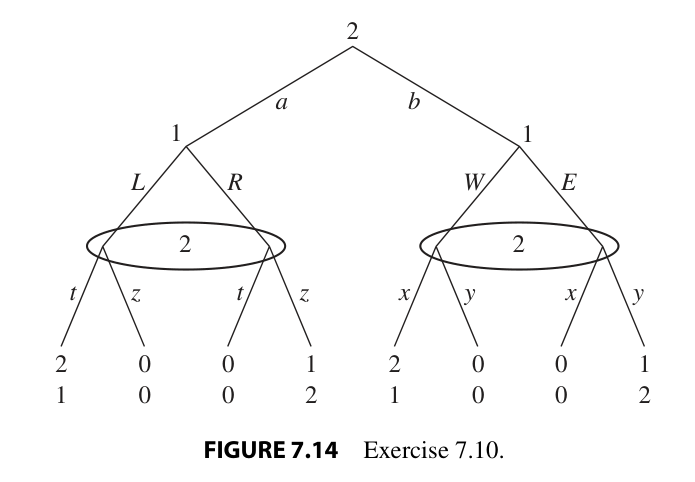
\includegraphics[keepaspectratio,alt={Figure 7.14 Exercise 7.10}]{../figures/tadelis-7-10.png}}



\begin{enumerate}

\def\labelenumi{\alph{enumi}.}

\item

  What are the pure-strategy sets for each player?

\item

  Show that for any behavioral strategy for player 1 there is a mixed strategy that leads to the same distribution over the terminal nodes regardless of the strategy chosen by player 2.

\item

  Show that for any behavioral strategy for player 2 there is a mixed strategy that leads to the same distribution over the terminal nodes regardless of the strategy chosen by player 1.

\item

  Now imagine that the game does not have perfect recall so that player 2's bottom two information sets are now one large information set. Can you find an example showing that the claim in (c) is no longer true?

\end{enumerate}

\end{quote}

